

\tikzset{every picture/.style={line width=0.75pt}} %set default line width to 0.75pt        

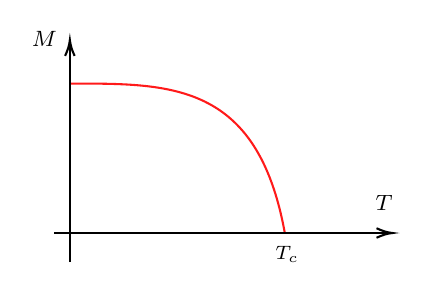
\begin{tikzpicture}[x=0.75pt,y=0.75pt,yscale=-1,xscale=1]
%uncomment if require: \path (0,130); %set diagram left start at 0, and has height of 130

%Curve Lines [id:da5736115837190213] 
\draw [color={rgb, 255:red, 255; green, 26; blue, 26 }  ,draw opacity=1 ]   (22.83,30) .. controls (71.17,30) and (113.17,29) .. (126.5,101.67) ;
%Straight Lines [id:da7029677561387601] 
\draw    (23,116) -- (23,11) ;
\draw [shift={(23,9)}, rotate = 90] [color={rgb, 255:red, 0; green, 0; blue, 0 }  ][line width=0.75]    (7.65,-2.3) .. controls (4.86,-0.97) and (2.31,-0.21) .. (0,0) .. controls (2.31,0.21) and (4.86,0.98) .. (7.65,2.3)   ;
%Straight Lines [id:da09730999984454025] 
\draw    (15.5,102) -- (176.4,102) ;
\draw [shift={(178.4,102)}, rotate = 180] [color={rgb, 255:red, 0; green, 0; blue, 0 }  ][line width=0.75]    (7.65,-2.3) .. controls (4.86,-0.97) and (2.31,-0.21) .. (0,0) .. controls (2.31,0.21) and (4.86,0.98) .. (7.65,2.3)   ;

% Text Node
\draw (3.17,3.57) node [anchor=north west][inner sep=0.75pt]  [font=\footnotesize]  {$M$};
% Text Node
\draw (168.87,82.4) node [anchor=north west][inner sep=0.75pt]  [font=\footnotesize]  {$T$};
% Text Node
\draw (120.52,107.02) node [anchor=north west][inner sep=0.75pt]  [font=\scriptsize]  {$T_{c}$};


\end{tikzpicture}
